\documentclass[11pt,letterpaper]{article}
\usepackage[spanish,es-noshorthands,es-tabla]{babel}
\usepackage[utf8]{inputenc}
\usepackage[T1]{fontenc}
\usepackage{lmodern}
\usepackage[margin=2.5cm]{geometry}
\usepackage{graphicx}
\usepackage{booktabs}
\usepackage{amsmath}
\usepackage{caption}
\usepackage{float}
\usepackage{microtype}
\usepackage[hidelinks]{hyperref}
\captionsetup{font=small,labelfont=bf}
\setlength{\parskip}{0.45em}
\setlength{\parindent}{0pt}
\renewcommand{\arraystretch}{1.15}

\begin{document}

\begin{titlepage}
\centering
{\large Universidad Externado de Colombia\\Facultad de Ciencia de Datos\par}
\vspace{3cm}
{\LARGE\bfseries Predicción de la rentabilidad de órdenes de transporte de carga en Colombia mediante regresión logística\par}
\vspace{1cm}
{\large Entrega final: modelo final, interpretación y despliegue\par}
\vspace{3cm}
{\large Integrantes:\\Daniel Pacheco\\Harold Burgos\par}
\vfill
{\large Asignatura: Machine Learning I\\Programa de Ciencia de Datos\par}
\end{titlepage}

\section{Introducción y recapitulación}

El proyecto adapta a Colombia el artículo de Grzelak et al. (2024) \cite{grzelak}, que usa una regresión logística para anticipar si una orden de transporte será rentable para una empresa pequeña en Polonia (AUC de 0,82 en entrenamiento y 0,81 en prueba, con punto de corte por Youden). Tomamos la metodología, no los coeficientes.

Al llegar una oferta de carga, el transportador conoce origen, destino, distancia, kilos, mercancía y naturaleza de la carga, pero el flete aún no está pactado. El modelo estima, solo con esas características, la probabilidad de que la orden termine pagada por debajo del costo de referencia. El valor pagado y el costo del SICE-TAC construyen la etiqueta y, en esta entrega, valoran en pesos cada error; nunca entran como predictores. Con precio cerrado basta compararlo con el costo; el modelo sirve antes, para priorizar y negociar.

Los datos cruzan el RNDC (lo pagado) con el SICE-TAC (costo eficiente por ruta) de diciembre de 2025 \cite{rndc,sicetac}, para camión rígido de dos ejes. Tras la limpieza de la segunda entrega quedan 20.868 viajes en 4.146 rutas, de los cuales el 67,7~\% cubre el costo de referencia. La clase positiva en todas las métricas y en los odds ratios es \emph{no rentable}. La partición es 80/20 agrupada por ruta y estratificada (16.695 viajes de entrenamiento y 4.173 de prueba), de modo que ninguna ruta queda en ambos lados; la prueba se usa una sola vez (sección~\ref{sec:prueba}).

\section{Modelo final y reproducción de los objetivos del artículo}

\subsection{Logaritmo o splines: la decisión}

En la segunda entrega la logística con kilómetros y kilos en logaritmo quedó como referencia, pero no cumplía la linealidad del logit: Box-Tidwell la rechazaba y Hosmer-Lemeshow fuera de muestra también, con una diferencia de hasta 5,9 puntos entre la proporción observada y la predicha por decil. La causa es visible: la proporción de viajes que cubren el costo cae de 81~\% en rutas de 7 a 8 horas de tránsito a 62~\% en las de 8 a 9, justo donde el mínimo de horas logísticas del costo pasa de 4 a 8 \cite{circular}. Una recta en el logaritmo de la distancia no sigue un salto; una curva por tramos sí. Por eso el candidato alterno usa splines cúbicos sobre el logaritmo de cada variable numérica.

Para decidir evaluamos ambos modelos, y KNN (el de mayor AUC en la segunda entrega), en los mismos 10 folds agrupados por ruta (Tabla~\ref{tab:decision} y Figura~\ref{fig:decision}). Nodos y regularización de los splines se eligieron por grilla en esa validación (6 nodos, $C = 0{,}1$).

\begin{table}[H]
\centering
\small
\caption{Comparación en los mismos 10 folds agrupados por ruta, con probabilidades fuera de muestra. PR-AUC de la clase no rentable. Desviación máxima: mayor diferencia entre proporción observada y predicha por decil.}
\label{tab:decision}
\begin{tabular}{lccccc}
\toprule
Modelo & AUC (media $\pm$ d.~e.) & PR-AUC & Brier & Hosmer-Lemeshow & Desv. máxima \\
\midrule
Logística con logaritmo & 0,775 $\pm$ 0,021 & 0,595 & 0,176 & 107,7 & 5,9 puntos \\
Logística con splines & 0,798 $\pm$ 0,016 & 0,636 & 0,166 & 33,7 & 3,7 puntos \\
KNN ($k = 61$) & 0,788 $\pm$ 0,018 & 0,625 & 0,169 & 50,3 & 3,6 puntos \\
\bottomrule
\end{tabular}
\end{table}

\begin{figure}[H]
\centering
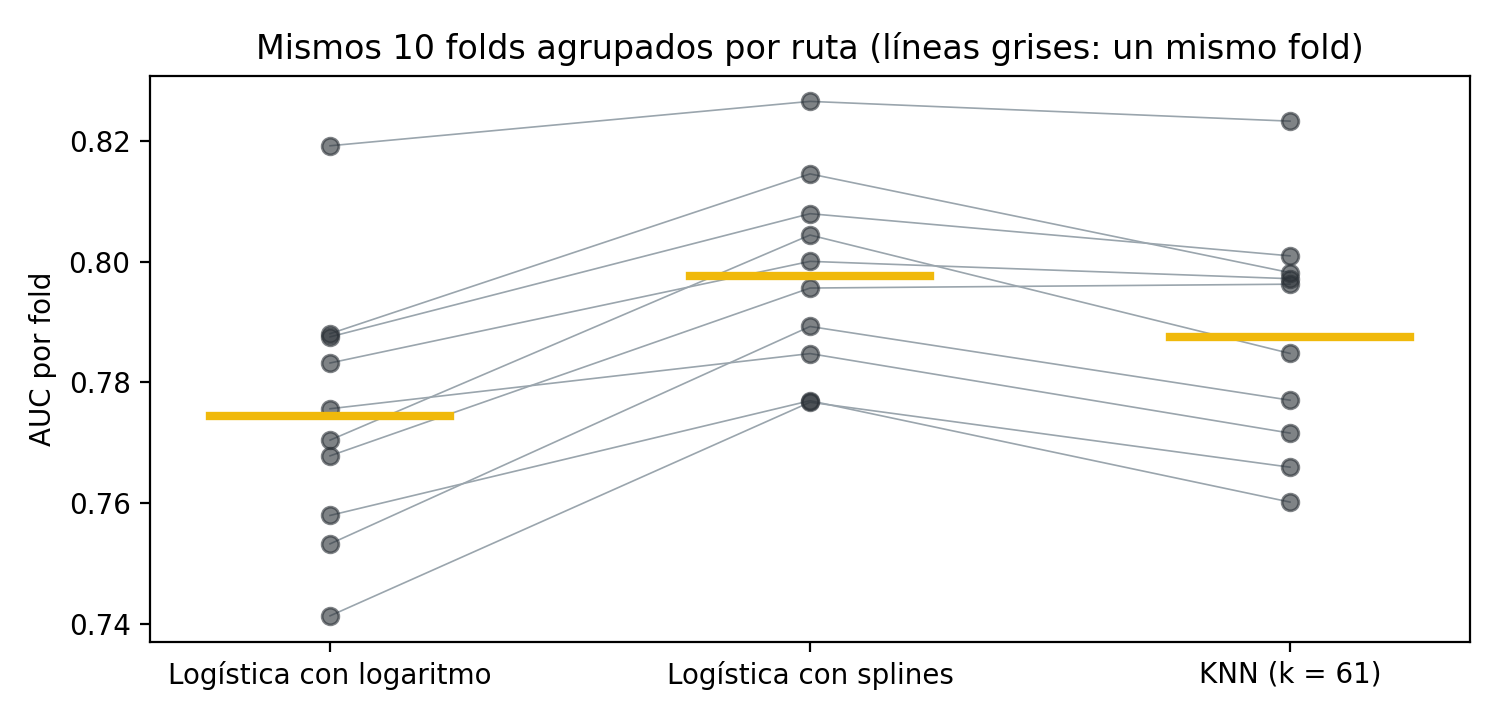
\includegraphics[width=0.66\textwidth]{fig_decision_modelo.png}
\caption{AUC por fold de los tres candidatos. Cada línea gris une el mismo fold; la barra amarilla es la media.}
\label{fig:decision}
\end{figure}

El modelo definitivo es la \textbf{regresión logística con splines}. Según la Tabla~\ref{tab:decision}, es la mejor en AUC, PR-AUC y Brier y la más estable entre folds. La Figura~\ref{fig:decision} muestra que la ventaja no depende de la partición: las líneas grises suben del logaritmo a los splines en los 10 folds, con una diferencia media de 0,023 de AUC (prueba $t$ pareada, $p = 0{,}0001$), y frente a KNN los splines ganan en 9 de 10 folds por 0,010. Además corrige en buena parte el supuesto que fallaba: Hosmer-Lemeshow baja de 107,7 a 33,7 y la desviación máxima por decil de 5,9 a 3,7 puntos. La calibración importa porque el umbral por costo usa el valor de la probabilidad y no solo el orden de los viajes. Frente a KNN, que rinde parecido, conserva la interpretación en odds ratios; a cambio, kilómetros y kilos se resumen en una curva y no en un único odds ratio (sección~\ref{sec:interp}).

\subsection{Evaluación en el conjunto de prueba}
\label{sec:prueba}

Con hiperparámetros y umbral ya fijados, el modelo se ajustó con todo el entrenamiento y se evaluó una sola vez sobre los 4.173 viajes reservados. El AUC es \textbf{0,784}, con intervalo de confianza del 95~\% de 0,766 a 0,801 por bootstrap de rutas completas, porque los viajes de una ruta no son independientes. El PR-AUC de la clase no rentable es 0,628, casi el doble de su prevalencia (0,323), y el Brier es 0,170. En la Figura~\ref{fig:prueba}, la curva ROC de prueba queda apenas por debajo de la de entrenamiento fuera de muestra (0,797), una caída de 0,013 sin sobreajuste relevante, y los deciles de calibración siguen la diagonal, con leve sobrestimación del riesgo entre 0,3 y 0,5 de probabilidad predicha.

\begin{figure}[H]
\centering
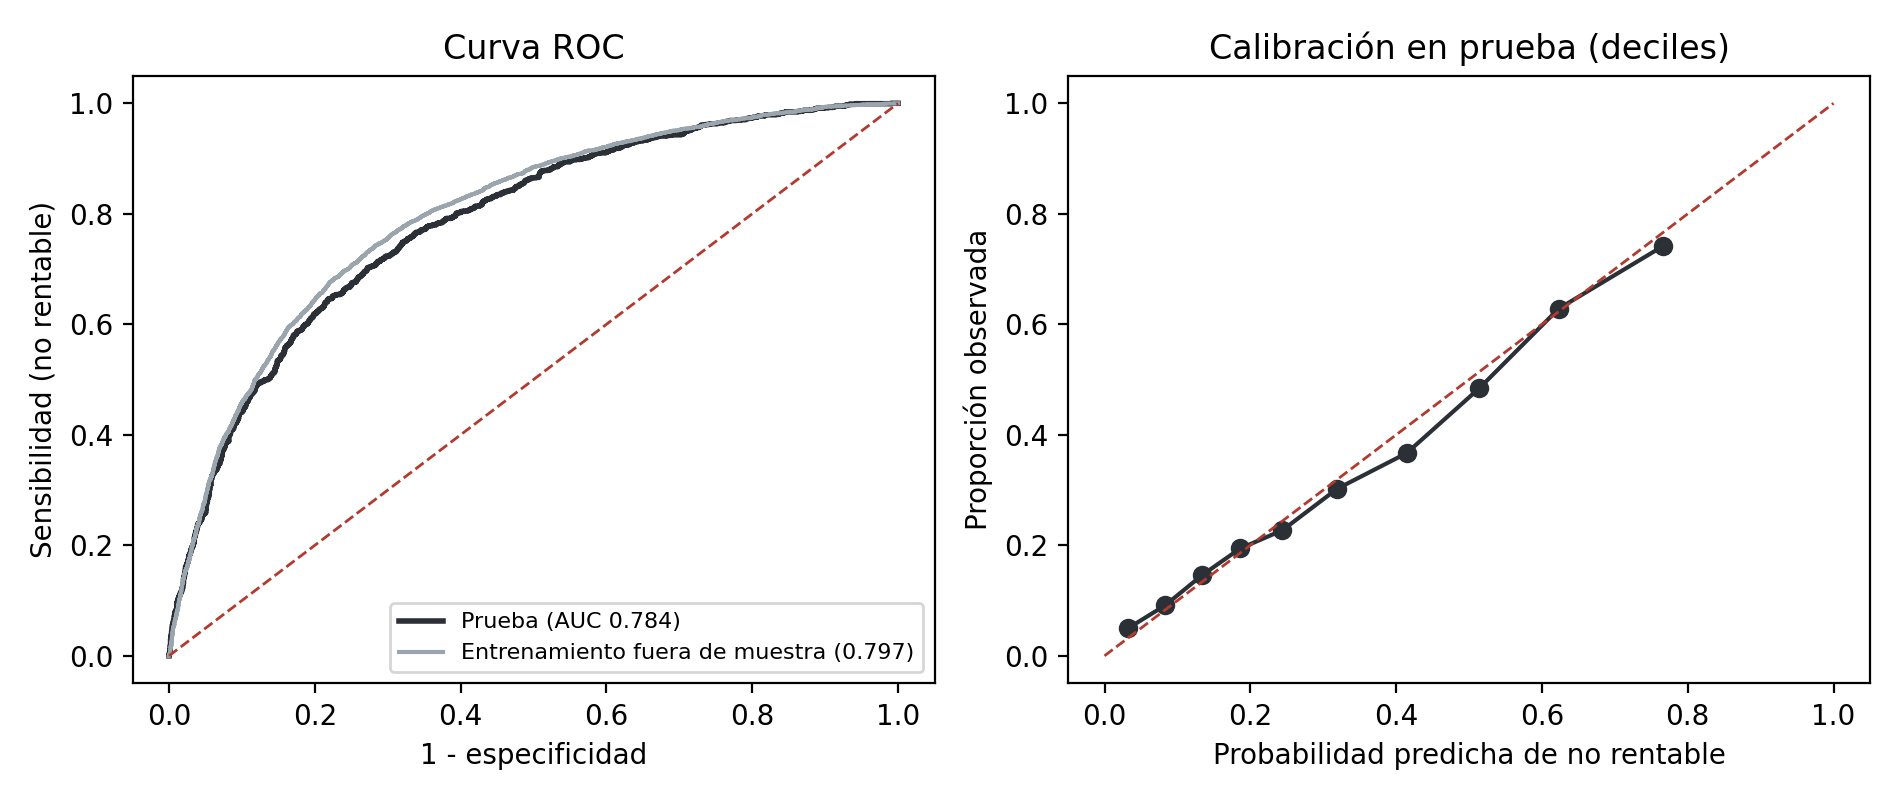
\includegraphics[width=0.80\textwidth]{fig_prueba_final.png}
\caption{Conjunto de prueba. Izquierda: curva ROC en prueba y en entrenamiento fuera de muestra. Derecha: proporción observada de viajes no rentables frente a la probabilidad predicha, por deciles.}
\label{fig:prueba}
\end{figure}

\subsection{Contraste con el artículo}

Se reprodujo el flujo del artículo. Nuestro AUC en prueba (0,784) es cercano al suyo (0,81), aunque menor: 0,81 supera el límite superior de nuestro intervalo. Sensibilidad y precisión no son comparables, porque su clase positiva es la orden rentable.

Las diferencias tienen explicación. El país es otro, los camiones son rígidos de dos ejes y no vehículos de hasta 3,5 toneladas, y los despachos son de muchas empresas y no el historial de una. Su etiqueta sale de la contabilidad de la empresa; la nuestra compara el pago con un costo de referencia oficial, que es una aproximación. El artículo define la orden rentable con un monto fijo (500 PLN) y usa como predictores el kilometraje diario, la velocidad, el consumo de combustible y el tiempo de operación, que solo se conocen después del viaje; nosotros usamos un costo propio de cada ruta y solo lo disponible al llegar la oferta. Además, el mes no varía. La validación es más estricta, porque al agrupar por ruta el modelo se evalúa siempre en corredores que no vio. Y donde el artículo no rechazó la linealidad del logit, aquí sí, lo que motivó los splines.

\section{Umbral desde el costo del negocio}

El índice de Youden, que usa el artículo, pesa igual los dos errores, pero aquí no cuestan lo mismo y el archivo de auditoría permite medirlos en pesos. Marcar una oferta es no aceptarla como viene (rechazarla o pedir más flete). Aceptar un viaje no rentable (falso negativo) cuesta el faltante, el costo menos el pago. Marcar un viaje rentable (falso positivo) pone en riesgo el margen, el pago menos el costo, pero tras la contraoferta el viaje puede conservarse; por eso se multiplica por $\alpha$, la fracción del margen que se pierde al marcar. El costo total de un umbral $u$ es
\[
\text{Costo}(u) = \sum_{\text{FN}(u)} (\text{costo} - \text{pago}) \; + \; \alpha \sum_{\text{FP}(u)} (\text{pago} - \text{costo}),
\]
y se elige el umbral que lo minimiza sobre las probabilidades fuera de muestra del entrenamiento, sin tocar la prueba.

En el entrenamiento, el faltante medio de un viaje no rentable es \$348.253 y el margen medio de un viaje rentable es \$468.662 (razón de 0,74). El caso base es $\alpha = 0{,}5$: la mitad de las ofertas marcadas se pierde y la otra mitad se conserva. Es un supuesto y no un dato, porque el RNDC no registra negociaciones; por eso se reporta la sensibilidad a $\alpha = 0{,}25$ y a $\alpha = 1$ (rechazar siempre). El umbral que minimiza el costo con $\alpha = 0{,}5$ es \textbf{0,44}.

\begin{table}[H]
\centering
\small
\caption{Umbrales candidatos sobre probabilidades fuera de muestra del entrenamiento. Sensibilidad y precisión de la clase no rentable. El costo por oferta y el ahorro frente a aceptar todas las ofertas se calculan con el $\alpha$ de cada fila (0,5 en las dos primeras), así que solo son comparables entre filas con el mismo $\alpha$.}
\label{tab:umbrales}
\begin{tabular}{lcccccc}
\toprule
Criterio & Umbral & Sensib. & Precisión & Marcadas & Costo por oferta & Ahorro \\
\midrule
Por defecto & 0,500 & 0,510 & 0,664 & 24,8~\% & \$51.663 & 54,1~\% \\
Youden (artículo) & 0,319 & 0,743 & 0,556 & 43,2~\% & \$58.691 & 47,8~\% \\
Costo, $\alpha = 0{,}5$ (elegido) & 0,440 & 0,599 & 0,631 & 30,7~\% & \$49.836 & 55,7~\% \\
\midrule
Costo, $\alpha = 0{,}25$ & 0,375 & 0,678 & 0,592 & 37,0~\% & \$34.353 & 69,5~\% \\
Costo, $\alpha = 1$ & 0,575 & 0,396 & 0,712 & 17,9~\% & \$69.373 & 38,4~\% \\
\bottomrule
\end{tabular}
\end{table}

\begin{figure}[H]
\centering
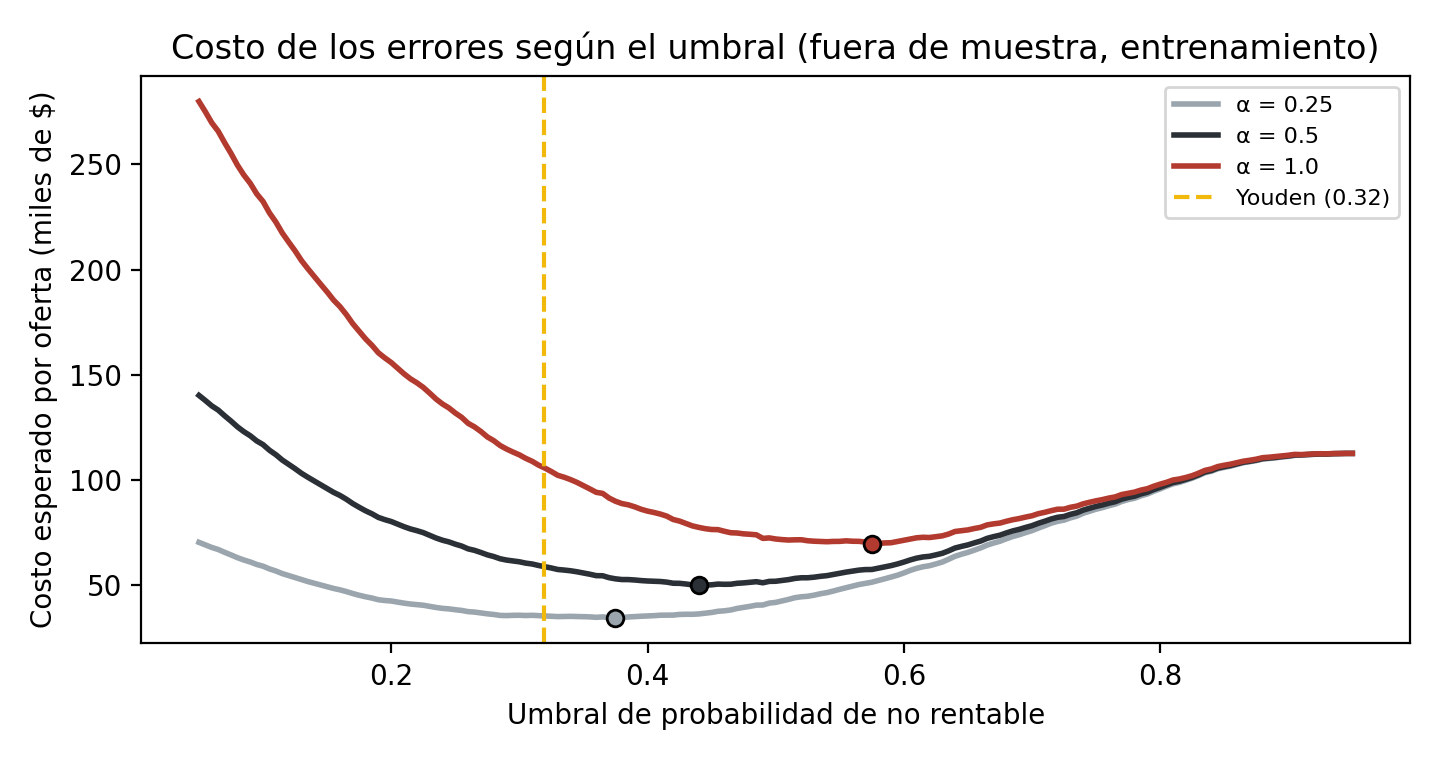
\includegraphics[width=0.66\textwidth]{fig_costo_umbral.png}
\caption{Costo esperado por oferta según el umbral, para tres valores de $\alpha$ (el punto marca el mínimo de cada curva), y umbral de Youden.}
\label{fig:costo}
\end{figure}

En la Tabla~\ref{tab:umbrales}, el umbral de Youden (0,319) detecta más viajes no rentables, pero marca el 43,2~\% de las ofertas y sacrifica margen de viajes buenos: cuesta \$58.691 por oferta frente a \$49.836 del umbral por costo. La Figura~\ref{fig:costo} muestra la sensibilidad al supuesto: el mínimo se desplaza de 0,375 a 0,575 cuando $\alpha$ pasa de 0,25 a 1, y Youden queda a la izquierda de los tres mínimos, es decir, marca de más en todo el rango considerado.

En prueba el resultado se mantiene (Tabla~\ref{tab:prueba}): con el umbral de 0,44 el modelo cuesta \$56.328 por oferta y evita el 48,7~\% de la pérdida de aceptar todo, frente a \$66.806 y 39,2~\% con Youden. En la matriz de confusión (Tabla~\ref{tab:confusion}), de 1.349 viajes no rentables se detectan 818 y pasan 531, y se marcan 544 viajes rentables: seis de cada diez ofertas marcadas eran efectivamente no rentables.

\begin{table}[H]
\centering
\small
\caption{Resultados en el conjunto de prueba según el umbral, con $\alpha = 0{,}5$.}
\label{tab:prueba}
\begin{tabular}{lcccccc}
\toprule
Criterio & Umbral & Sensib. & Precisión & Marcadas & Costo por oferta & Ahorro \\
\midrule
Costo, $\alpha = 0{,}5$ (elegido) & 0,440 & 0,606 & 0,601 & 32,6~\% & \$56.328 & 48,7~\% \\
Youden (artículo) & 0,319 & 0,733 & 0,529 & 44,8~\% & \$66.806 & 39,2~\% \\
Por defecto & 0,500 & 0,514 & 0,628 & 26,4~\% & \$57.943 & 47,2~\% \\
\bottomrule
\end{tabular}
\end{table}

\begin{table}[H]
\centering
\small
\caption{Matriz de confusión en prueba con el umbral de 0,44.}
\label{tab:confusion}
\begin{tabular}{lcc}
\toprule
 & Modelo: aceptar & Modelo: marcar \\
\midrule
Real: rentable & 2.280 & 544 \\
Real: no rentable & 531 & 818 \\
\bottomrule
\end{tabular}
\end{table}

\section{Interpretación de resultados}
\label{sec:interp}

\subsection{Factores influyentes en odds}

Para interpretar estimamos con statsmodels \cite{statsmodels} una logística sin regularización, con los mismos splines, categorías de referencia explícitas y errores estándar agrupados por ruta (pseudo $R^2$ de McFadden de 0,221). Un odds ratio (OR) mayor que 1 significa más \emph{odds} de que el viaje no cubra el costo frente a la referencia; no es un cambio en la probabilidad, que depende del punto de partida.

La carga refrigerada tiene un OR de 3,75 (IC del 95~\%: 2,78 a 5,06) frente a la carga normal, a igualdad de lo demás. Un ejemplo muestra la diferencia: si un viaje de carga normal tiene una probabilidad de 20~\% de no cubrir el costo (odds de 0,25), el mismo viaje refrigerado tiene odds de $0{,}25 \times 3{,}75 \approx 0{,}94$, es decir, una probabilidad de 48~\%; si la de partida fuera 50~\%, pasaría a 79~\%. En ningún caso la probabilidad se multiplica por 3,75. La carga peligrosa ya no se distingue de la normal (OR de 0,80; IC de 0,58 a 1,09), lo que respalda la sospecha de la segunda entrega de que su aparente menor riesgo era un artefacto del costo asignado.

Kilómetros y kilos se leen como curvas de OR frente a un viaje mediano, de 375 km y 4.500 kg (Figura~\ref{fig:or} y Tabla~\ref{tab:orkm}). La distancia tiene tres zonas. Hasta unos 200 km las odds de no cubrir el costo son entre la sexta y la quinta parte de las del viaje mediano (OR de 0,15 a 0,21). Entre 200 y 400 km suben con rapidez: el OR pasa de 0,54 a 300 km a 1,13 a 400 km, es decir, las odds se duplican en 100 km. Ese es el salto que el logaritmo no podía representar y que coincide con el cambio de 4 a 8 horas logísticas. Por encima de 400 km el OR se estabiliza entre 1,1 y 1,3 y sube en las rutas más largas (1,52 a 1.000 km). El peso actúa en sentido contrario: en el panel derecho de la Figura~\ref{fig:or} una carga de 500 kg tiene un OR de 2,69 (IC 95 % 2,31 a 3,13) frente a la mediana, y una de 10.000 kg uno de 0,15 (0,12 a 0,18). El flete crece con las toneladas, mientras que el costo de referencia depende de la ruta y no de cuánto se cargue.

\begin{figure}[H]
\centering
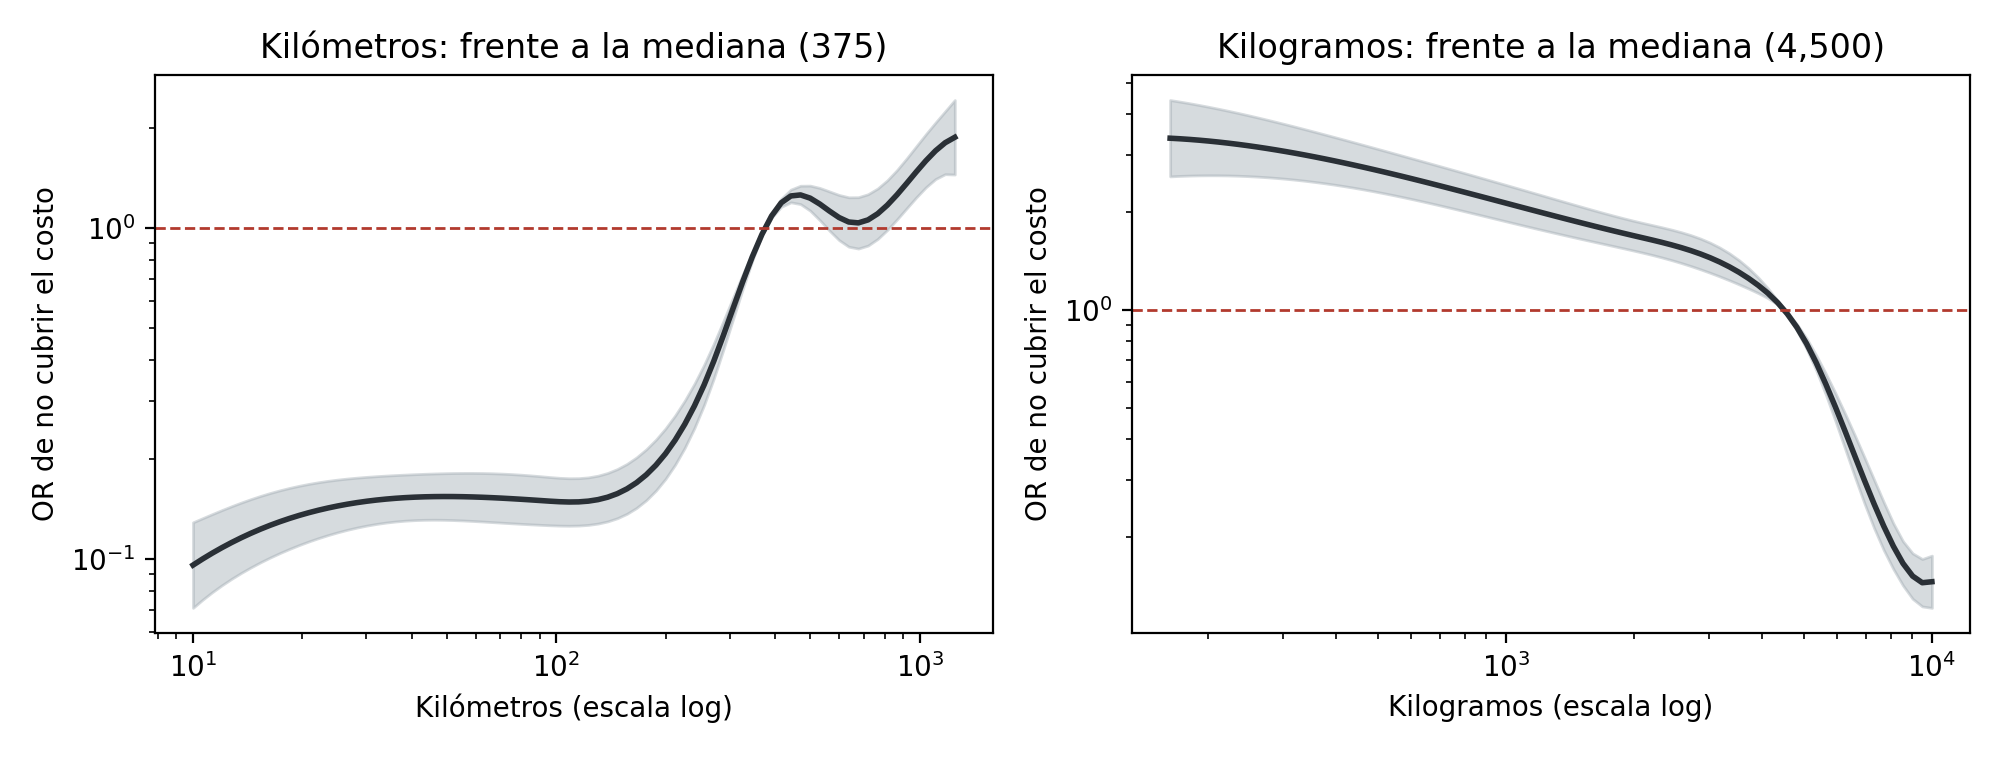
\includegraphics[width=0.88\textwidth]{fig_or_curvas.png}
\caption{Odds ratio de no cubrir el costo frente a un viaje mediano, con banda de confianza del 95~\%. Ejes en escala logarítmica.}
\label{fig:or}
\end{figure}

\begin{table}[H]
\centering
\small
\caption{Odds ratio de no cubrir el costo según la distancia, frente a un viaje de 375 km (IC del 95~\% con errores agrupados por ruta).}
\label{tab:orkm}
\begin{tabular}{lcccccccc}
\toprule
Kilómetros & 50 & 100 & 200 & 300 & 400 & 500 & 600 & 1.000 \\
\midrule
OR & 0,15 & 0,15 & 0,21 & 0,54 & 1,13 & 1,23 & 1,07 & 1,52 \\
IC inferior & 0,13 & 0,13 & 0,18 & 0,49 & 1,11 & 1,13 & 0,92 & 1,27 \\
IC superior & 0,18 & 0,18 & 0,25 & 0,58 & 1,15 & 1,34 & 1,26 & 1,82 \\
\bottomrule
\end{tabular}
\end{table}

\subsection{Tipos de error y significado práctico}

Los errores de prueba no se reparten al azar (Tabla~\ref{tab:errores}). Hasta 100 km el modelo acierta el 85,5~\% y casi nunca marca un viaje rentable (1,1~\%); el error típico es dejar pasar uno no rentable (13,4~\%). De 400 a 600 km el acierto baja a 67,1~\% y el error dominante se invierte: se marca el 24,6~\% de los viajes aunque eran rentables. Allí la respuesta razonable es una contraoferta, más que un rechazo.

\begin{table}[H]
\centering
\small
\caption{Aciertos y errores en prueba (umbral de 0,44), por tramo de distancia y por cercanía al punto de equilibrio. Porcentajes por fila.}
\label{tab:errores}
\begin{tabular}{lccc}
\toprule
Grupo & Acierto & Falso negativo & Falso positivo \\
\midrule
Hasta 100 km & 85,5~\% & 13,4~\% & 1,1~\% \\
100 a 250 km & 82,2~\% & 15,9~\% & 1,9~\% \\
250 a 400 km & 74,1~\% & 13,3~\% & 12,6~\% \\
400 a 600 km & 67,1~\% & 8,3~\% & 24,6~\% \\
Más de 600 km & 65,6~\% & 15,4~\% & 18,9~\% \\
\midrule
Pago a más de 10~\% del costo & 80,5~\% & 8,6~\% & 10,9~\% \\
Pago a $\pm$10~\% del costo & 54,6~\% & 25,6~\% & 19,8~\% \\
\bottomrule
\end{tabular}
\end{table}

El segundo patrón es la cercanía al punto de equilibrio. Solo el 24,1~\% de los viajes de prueba se pagó entre 0,9 y 1,1 veces el costo, pero allí está el 42,5~\% de los errores; en esa franja el modelo acierta el 54,6~\% de las veces, y fuera de ella el 80,5~\%. Son los errores más baratos, porque el monto en juego es pequeño, y los más discutibles, porque allí la etiqueta depende de la aproximación del costo.

Para un transportador, una oferta corta y pesada rara vez queda por debajo del costo, y una de más de 400 km, liviana o refrigerada, merece revisar el flete antes de aceptar. La salida es una probabilidad para priorizar y negociar, no un veredicto: con el umbral elegido, cuatro de cada diez ofertas marcadas habrían cubierto el costo.

\section{Despliegue básico}

El modelo se desplegó como una aplicación de Streamlit \cite{streamlit}, RutaRentable, pensada para el transportador individual. El usuario elige municipio de origen y destino (el departamento se deduce), la mercancía por su nombre (la aplicación la traduce al capítulo que usa el modelo), los kilos y el tipo de carga; los kilómetros se completan con la distancia oficial de la ruta en el SICE-TAC o, si la ruta no existe, con una estimación editable. La respuesta se da en lenguaje llano: un semáforo, la frase ``de cada 10 viajes como este, unos N no alcanzaron a cubrir el costo y los factores que más pesan en esa oferta; la probabilidad, las odds y el umbral (0,44 por defecto, Youden o personalizado) quedan como detalle técnico. Junto al riesgo, la aplicación muestra el costo de referencia SICE-TAC de la ruta, el rango pagado en viajes parecidos del RNDC y, si el usuario escribe el precio ofrecido, si este cubre el costo. Esos valores nunca entran al modelo: el riesgo sirve antes de tener precio y la comparación directa, después. Una pestaña compara varias ofertas y otra procesa un CSV para empresas transportadoras. En la Figura~\ref{fig:app}, una oferta de 4.500 kg de Bogotá a Medellín (429 km oficiales) recibe 61,9~\% de probabilidad de no cubrir el costo, odds de 1,62 a 1; como supera el umbral, la recomendación es pedir más flete.

La coherencia entre entrenamiento y uso se garantiza de tres formas. Primero, se guarda el \texttt{Pipeline} completo ya ajustado (imputación, logaritmo, splines, estandarización, one-hot y regresión logística), de modo que la aplicación no reimplementa ninguna transformación. Segundo, el archivo desplegado es el modelo evaluado en la prueba: el notebook verifica que, recargado, produce las mismas probabilidades. Tercero, \texttt{metadatos.json} guarda el umbral, los rangos de kilómetros y kilos del entrenamiento y las categorías válidas; la aplicación solo ofrece categorías conocidas y advierte cuando una entrada cae fuera del rango visto, donde la predicción es una extrapolación.

Está publicada en \url{https://ruta-rentable.streamlit.app} (Streamlit Community Cloud) y en local se ejecuta con \texttt{pip install -r requirements.txt} y \texttt{streamlit run app.py} desde la carpeta de la aplicación.

\IfFileExists{captura_app.png}{%
\begin{figure}[H]
\centering
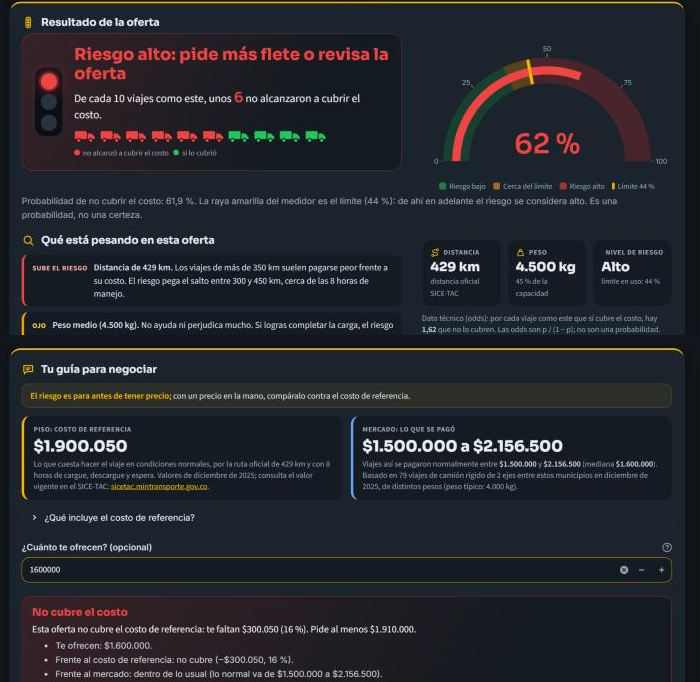
\includegraphics[width=0.80\textwidth]{captura_app.png}
\caption{Aplicación RutaRentable: datos de la oferta por municipio y mercancía, mapa de la ruta, semáforo con la frecuencia natural y medidor de la probabilidad frente al umbral.}
\label{fig:app}
\end{figure}
}{}

\section{Calidad, limitaciones y proyección}

\textbf{Un solo mes.} Los datos son solo de diciembre de 2025. La variable mes, significativa en el artículo, no pudo usarse, y la validación por ruta mide la generalización a corredores nuevos, no a meses nuevos. El paso más importante es validar fuera de tiempo: entrenar con diciembre y evaluar con otro mes.

\textbf{Etiqueta aproximada.} El costo de referencia supone una carrocería (si se asume furgón cambia la etiqueta de 8,1~\% de los viajes), usa el mínimo de horas logísticas y asigna el costo de carga general a la carga peligrosa. Con etiquetas alternativas el AUC se sostuvo en la segunda entrega: el orden de los viajes es robusto, pero la clasificación cerca del equilibrio es frágil. Además, cubrir un costo eficiente no es obtener utilidad: el costo real de cada transportador puede ser distinto.

\textbf{Alcance y representatividad.} Los resultados aplican a camiones rígidos de dos ejes y a rutas que el SICE-TAC costea. El conjunto excluye las filas del RNDC que agrupan varios viajes, por lo que subrepresenta los corredores de mayor volumen, y parte del efecto de la distancia refleja una regla del costo, no solo el mercado.

\textbf{Solo viajes ejecutados.} El RNDC registra los viajes que se hicieron; las ofertas rechazadas no quedan, así que el riesgo de las peores ofertas puede estar subestimado. Un piloto que registre todas las ofertas recibidas permitiría corregirlo.

\textbf{Supuestos y umbral.} Hosmer-Lemeshow sigue rechazando el ajuste con los splines; con 16.695 viajes detecta desviaciones pequeñas (la máxima por decil es de 3,7 puntos), pero la calibración no es perfecta. La dependencia entre viajes de una ruta se atendió agrupando la validación, los errores estándar y el bootstrap. El umbral depende de $\alpha$, que es un supuesto, y los costos de los errores se midieron sobre la misma etiqueta aproximada.

\textbf{Proyección hacia Machine Learning II.} Cinco líneas dan continuidad: un modelo del pago (por ejemplo, regresión del logaritmo del flete) que estime qué tan seguido se paga al menos un valor dado; modelos aditivos generalizados con penalización, que eligen la suavidad de las curvas en lugar de fijar los nodos; ensambles de árboles como \emph{gradient boosting}, que capturan interacciones entre ruta, peso y mercancía a cambio de interpretabilidad; calibración y aprendizaje sensible al costo, que lleva el costo de cada error al entrenamiento y no solo al umbral; y validación temporal con varios meses.

\section{Conclusiones}

La regresión logística con splines superó al logaritmo en los 10 folds, corrigió en buena parte la falta de linealidad y conservó la lectura en odds ratios. En prueba alcanzó un AUC de 0,784, cercano al 0,81 del artículo, y el umbral de 0,44, elegido por costo en pesos, evita más pérdida que el de Youden. La distancia, el peso y la carga refrigerada son los factores que más mueven el riesgo, y los errores se concentran cerca del punto de equilibrio. El modelo sirve para priorizar ofertas en camión rígido de dos ejes; extenderlo exige, ante todo, validarlo con otros meses.

\textbf{Código.} Se entregan los notebooks 01 a 04 y la aplicación con el modelo exportado. Todo el flujo usa la semilla 42 y se construyó con pandas \cite{pandas}, scikit-learn \cite{sklearn}, statsmodels y Streamlit; el mapa de la aplicación usa los centroides municipales de la DIVIPOLA \cite{divipola}. Código, datos y pruebas: \url{https://github.com/PachecoDa/RUTA-RENTABLE}.

\begin{thebibliography}{9}
\small
\bibitem{grzelak} Grzelak, M., Owczarek, P., Stoica, R.-M., Voicu, D., y Vil\u{a}u, R. (2024). Application of logistic regression to analyze the economic efficiency of vehicle operation in terms of the financial security of enterprises. \emph{Logistics}, 8(2), 46. \url{https://doi.org/10.3390/logistics8020046}
\bibitem{rndc} Ministerio de Transporte de Colombia. Registro Nacional de Despachos de Carga (RNDC). \url{https://plc.mintransporte.gov.co}
\bibitem{sicetac} Ministerio de Transporte de Colombia. Sistema de Información de Costos Eficientes para el Transporte Automotor de Carga (SICE-TAC). \url{https://sicetac.mintransporte.gov.co}
\bibitem{circular} Ministerio de Transporte de Colombia (2025, 3 de septiembre). Circular Externa 20251010000577: orientaciones frente a las horas logísticas mínimas establecidas en el SICE-TAC.
\bibitem{divipola} Departamento Administrativo Nacional de Estadística (DANE). Codificación de la División Político-Administrativa de Colombia (DIVIPOLA). \url{https://geoportal.dane.gov.co/geovisores/territorio/consulta-divipola-division-politico-administrativa-de-colombia/}
\bibitem{pandas} McKinney, W. (2010). Data structures for statistical computing in Python. En \emph{Proceedings of the 9th Python in Science Conference}, 56--61. \url{https://doi.org/10.25080/Majora-92bf1922-00a}
\bibitem{sklearn} Pedregosa, F., Varoquaux, G., Gramfort, A., Michel, V., Thirion, B., Grisel, O., et al. (2011). Scikit-learn: Machine learning in Python. \emph{Journal of Machine Learning Research}, 12, 2825--2830.
\bibitem{statsmodels} Seabold, S., y Perktold, J. (2010). Statsmodels: Econometric and statistical modeling with Python. En \emph{Proceedings of the 9th Python in Science Conference}, 92--96. \url{https://doi.org/10.25080/Majora-92bf1922-011}
\bibitem{streamlit} Streamlit (2026). Streamlit: A faster way to build and share data apps (versión 1.67). \url{https://streamlit.io}
\end{thebibliography}

\noindent\small\textit{Declaración de uso de IA generativa.} Usamos un asistente de IA generativa (Claude, de Anthropic) como apoyo en esta entrega: para escribir y depurar el notebook final y la aplicación, y para redactar un primer borrador de este informe. El equipo ejecutó el código, verificó cada cifra contra las salidas de los notebooks, tomó las decisiones técnicas (modelo, umbral y supuesto de $\alpha$) y está en capacidad de explicarlas y defenderlas.

\end{document}
